\chapter{Benutzeroberfläche}
    Die Hauptaufgabe unserer GUI liegt darin Workflow-Anwendungen zu erstellen. Die Erstellung und Einsicht von Workflow-Anwendungen ist erst nachdem Anmelden sichtbar. Es gibt folgende Ansichten:
    \begin{itemize}
        \item Login/Logout [Abb. 1]
        \item Registrierung [Abb. 2]
        \item Admin [Abb. 3]
        \item Workflow design [Abb. 4]
        \item Workflow Ausführung [Abb. 5]
    \end{itemize}

    \begin{figure}[ht]
 \centering
 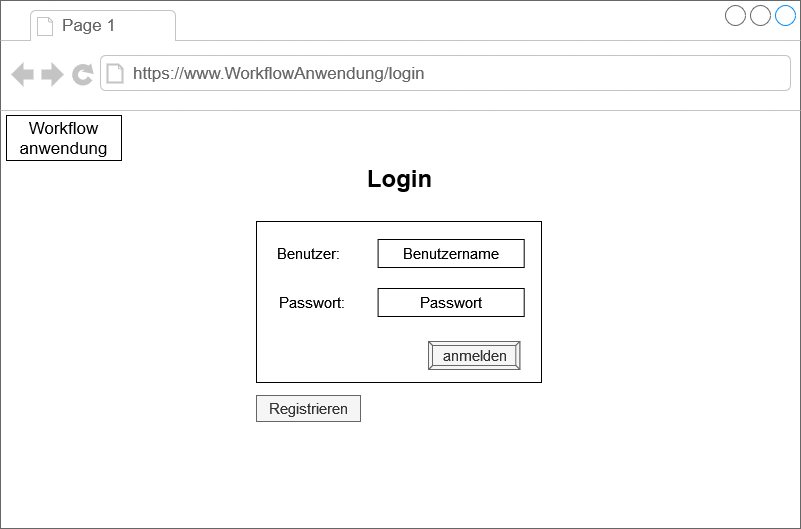
\includegraphics[width = 0.75\textwidth]{Grafiken/loginGui.drawio.png}
 \caption{Login Seite}
 \label{Abb 1}
\end{figure}

\begin{figure}[ht]
 \centering
 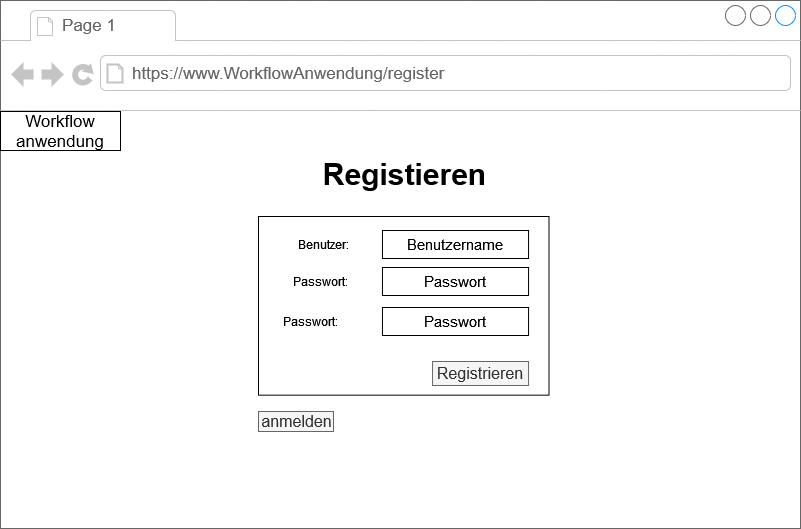
\includegraphics[width = 0.75\textwidth]{Grafiken/registrationGui.drawio.png}
 \caption{Registrierungsseite}
 \label{fig:Abb 2}
\end{figure}

\begin{figure}[ht]
 \centering
 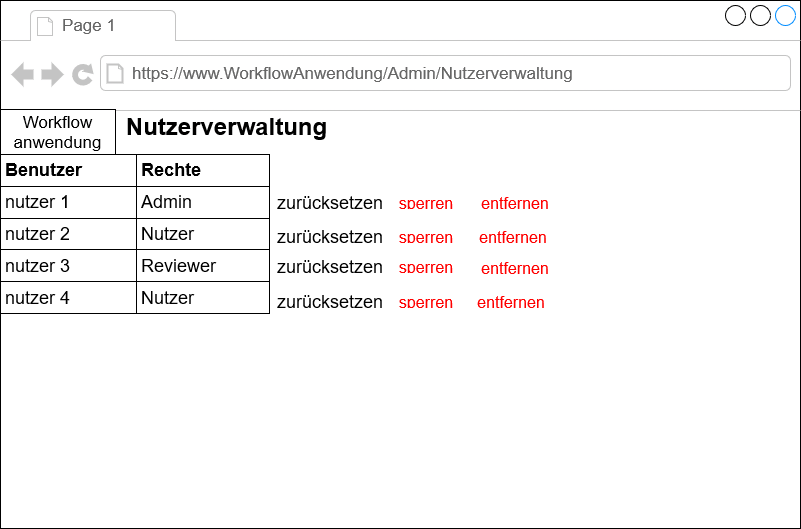
\includegraphics[width = 0.75\textwidth]{Grafiken/nutzerverwaltungGui.drawio.png}
 \caption{Nutzerverwaltung}
 \label{fig:Abb 3}
\end{figure}

\begin{figure}[ht]
 \centering
 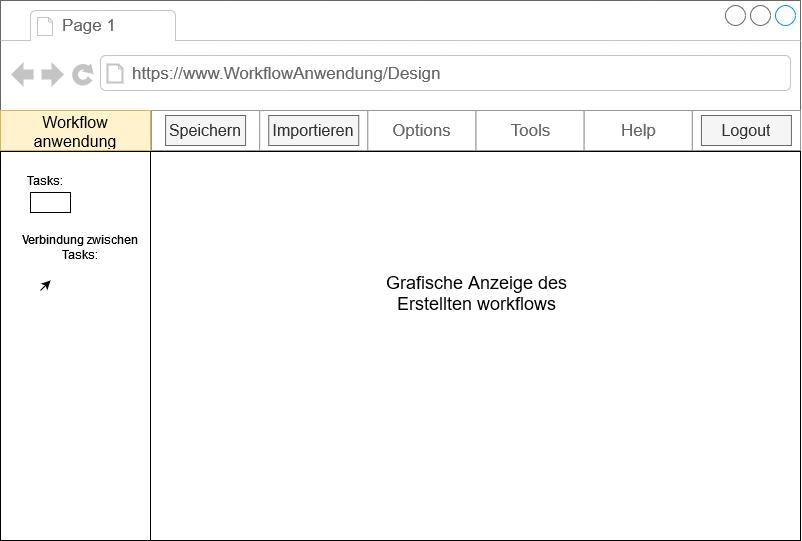
\includegraphics[width = 0.75\textwidth]{Grafiken/workflowDesignGui.drawio.png}
 \caption{Designen von Workflows}
 \label{fig:Abb 4}
\end{figure}
